%% Commands for TeXCount
%TC:macro \cite [option:text,text]
%TC:macro \citep [option:text,text]
%TC:macro \citet [option:text,text]
%TC:envir table 0 1
%TC:envir table* 0 1
%TC:envir tabular [ignore] word
%TC:envir displaymath 0 word
%TC:envir math 0 word
%TC:envir comment 0 0
%%
%%
%% The first command in your LaTeX source must be the \documentclass command.
\documentclass[sigconf ,nonacm]{acmart}

%%
%% \BibTeX command to typeset BibTeX logo in the docs
\AtBeginDocument{%
  \providecommand\BibTeX{{%
    \normalfont B\kern-0.5em{\scshape i\kern-0.25em b}\kern-0.8em\TeX}}}


\begin{document}


\title{Music Genre Classification}

\author{Ruochen Kong}
\email{ruochen.kong@emory.edu}
\affiliation{%
  \institution{Emory University}
  \city{Atlanta}
  \state{Georgia}
  \country{USA}
}

%%
%% Keywords. The author(s) should pick words that accurately describe
%% the work being presented. Separate the keywords with commas.
\keywords{Signal Processing, Data Mining, Machine Learning, Music Analysis}
\begin{abstract}
Searching music by genre is a function implemented in almost all music apps, so developing an accurate algorithm to classify the music is crucial. The existing research papers have successfully classified music into no more than 10 genres, but in the real world, much more detailed genres exist. This rough classification may further cause an unsatisfaction with the user experience. In this project, I investigated the signal of the music in 19 genres, extracted distinguishable features, and applied them to classification models. The result shows that, in general, the simple 2-layer CNN performs better than Random Forest, the normalized features perform better than original features, and a selection of features based on correlations improves the performance. 
\end{abstract}

\maketitle

\section{Introduction}
Major music applications, such as Spotify, Apple Music, or Gnoosic, have all allowed users to search by genre. The accuracy of the search result highly affects the satisfaction of users. The previous research has successfully developed models to classify music into 10 different genres with accuracy higher than 80\% evaluated on the GTZAN Dataset \cite{panagakis2009music,lee2009automatic,sigtia2014improved,fu2010survey}. These models, however, may not be as successful when facing more genres of datasets in the real world. According to Tamatjita et al. (2016), the performance of classification models drops significantly by increasing the number of genres from 6 to 12 \cite{comparison}. This drawback is understandable because the more the genres the more demanding the model is to detect differences between features, but pursuing a more accurate automatic classification method is still necessary. 

This project aims to establish a method to classify music into 19 genres with the dataset found on Kaggle\footnote{https://www.kaggle.com/competitions/kaggle-pog-series-s01e02}. The dataset contains 19.9k music labeled as \textit{Electronic, Rock, Punk, Experimental, Hip-Hop, Folk, Chiptune and Glitch, Instrumental, Pop, International, Ambient Electronic, Classical, Old-Time and Historic, Jazz, Country, Soul-RnB, Spoken, Blues, or Easy Listening.} To develop the model, I started with extracting features from raw signal data. Common audio features are considered, including beats, tuning, zero-crossing rate, autocorrelation, root mean square energy (RMS), centroid, flatness, Mel-frequency cepstral coefficient (MFCC), and short-time Fourier transformation (STFT) \cite{peeters2004large,muller2011signal,gtzan}. The extracted features are normalized and filtered by correlations \cite{yu2003feature}, and then applied with random forest (RF) and a 2-layer CNN. The overall accuracy of each model is higher than 45\% with the highest accuracy 47.6\% achieved by CNN with features both normalized and filtered. Hence, by comparison of the use of different models and different feature formats, a general conclusion is that CNN outperforms RF and normalized features outperform the original features. 

The rest of the report is organized as: Section 2 presents the related work on music classification based on audio signals. Section 3 provides an overview of the dataset. Features used in this project are extracted and selected in Section 4. Section 5 provides the experiment process and the results. The discussion of limitations and possible improvements is in section 6. A conclusion of the project is finally provided in section 7.


\section{Related Work}

In 2001, Tzanetakis et al. presented groundbreaking research in music classification \cite{gtzan}. The authors summarized the music features into three general types, (i) timbral texture features, (ii) rhythmic content features, and (iii) pitch content features. Timbral texture features include spectral centroid, spectral roll-off, spectral flux, zero crossings, MFCC, analysis windows, and low-energy features; rhythmic content features are mainly beat analysis by full-wave rectification, low-pass filtering, downsampling, mean removal, enhanced autocorrelation, peak detection, and histogram calculation, and beat histogram features; pitch content features are based on multiple pitch detections with the technic provided by Tolonen and Karjalainen in 2000 \cite{tolonen2000computationally}. The authors also developed a dataset, GTZAN, which is labeled hierarchically that allows classification tasks with both 10 genres and 20 genres. The GTZAN dataset has then been widely used in evaluations of the following research.


Several models have been developed and evaluated on the GTZAN dataset. Lee et al. (2009) and Fu et al. (2010) achieved classification accuracy slightly higher than 90\% both with MFCC, amplitude spectrum envelop (ASE) and octave based spectral contrast (OSC) \cite{lee2009automatic,fu2010feature}. Li et al. (2010) reported accuracy of 84\% by CNN with majority votes \cite{li2010automatic}. Feng (2014) reported accuracy of 61\% with a 5-layer Restricted Boltzam Machine (RBM) \cite{feng2014deep}. 


Finally, Tamatjita et al. (2016) presented a comparison of different numbers of genres to be classified \cite{comparison}. The authors used Nearest Centroid Classifier as their model with the same audio features to classify music into 3, 6, 9, and 12 genres. They used 120 songs as test data and reported an accuracy of 96.7\% on 3 genres, 70\% on 6 genres, 53.3\% on 9 genres, and 33.3\% on 12 genres.

\section{Dataset}
The dataset contains 19922 ogg files with 3071 in Electronic, 3095 in Rock, 2582 in Punk, 1800 in Experimental, 1757 in Hip-Hop, 1241 in Folk, 1181 in Chiptune and Glitch, 1044 in Instrumental, 945 in Pop, 814 in International, 796 in Ambient Electronic, 495 in Classical, 408 in Old-Time and Historic, 306 in Jazz, 142 in Country, 94 in Soul-RnB, 94 in Spoken, 58 in Blues, and 13 in Easy Listening. The corresponding genre ids are in the same order starting from 0. The genre was annotated by humans which may include errors. Each music segment is around 30 seconds with slight differences and contains 2 channels. Figure \ref{fig:elec} and \ref{fig:intru} represents an example of electronic music and instrumental music.
\begin{figure}
  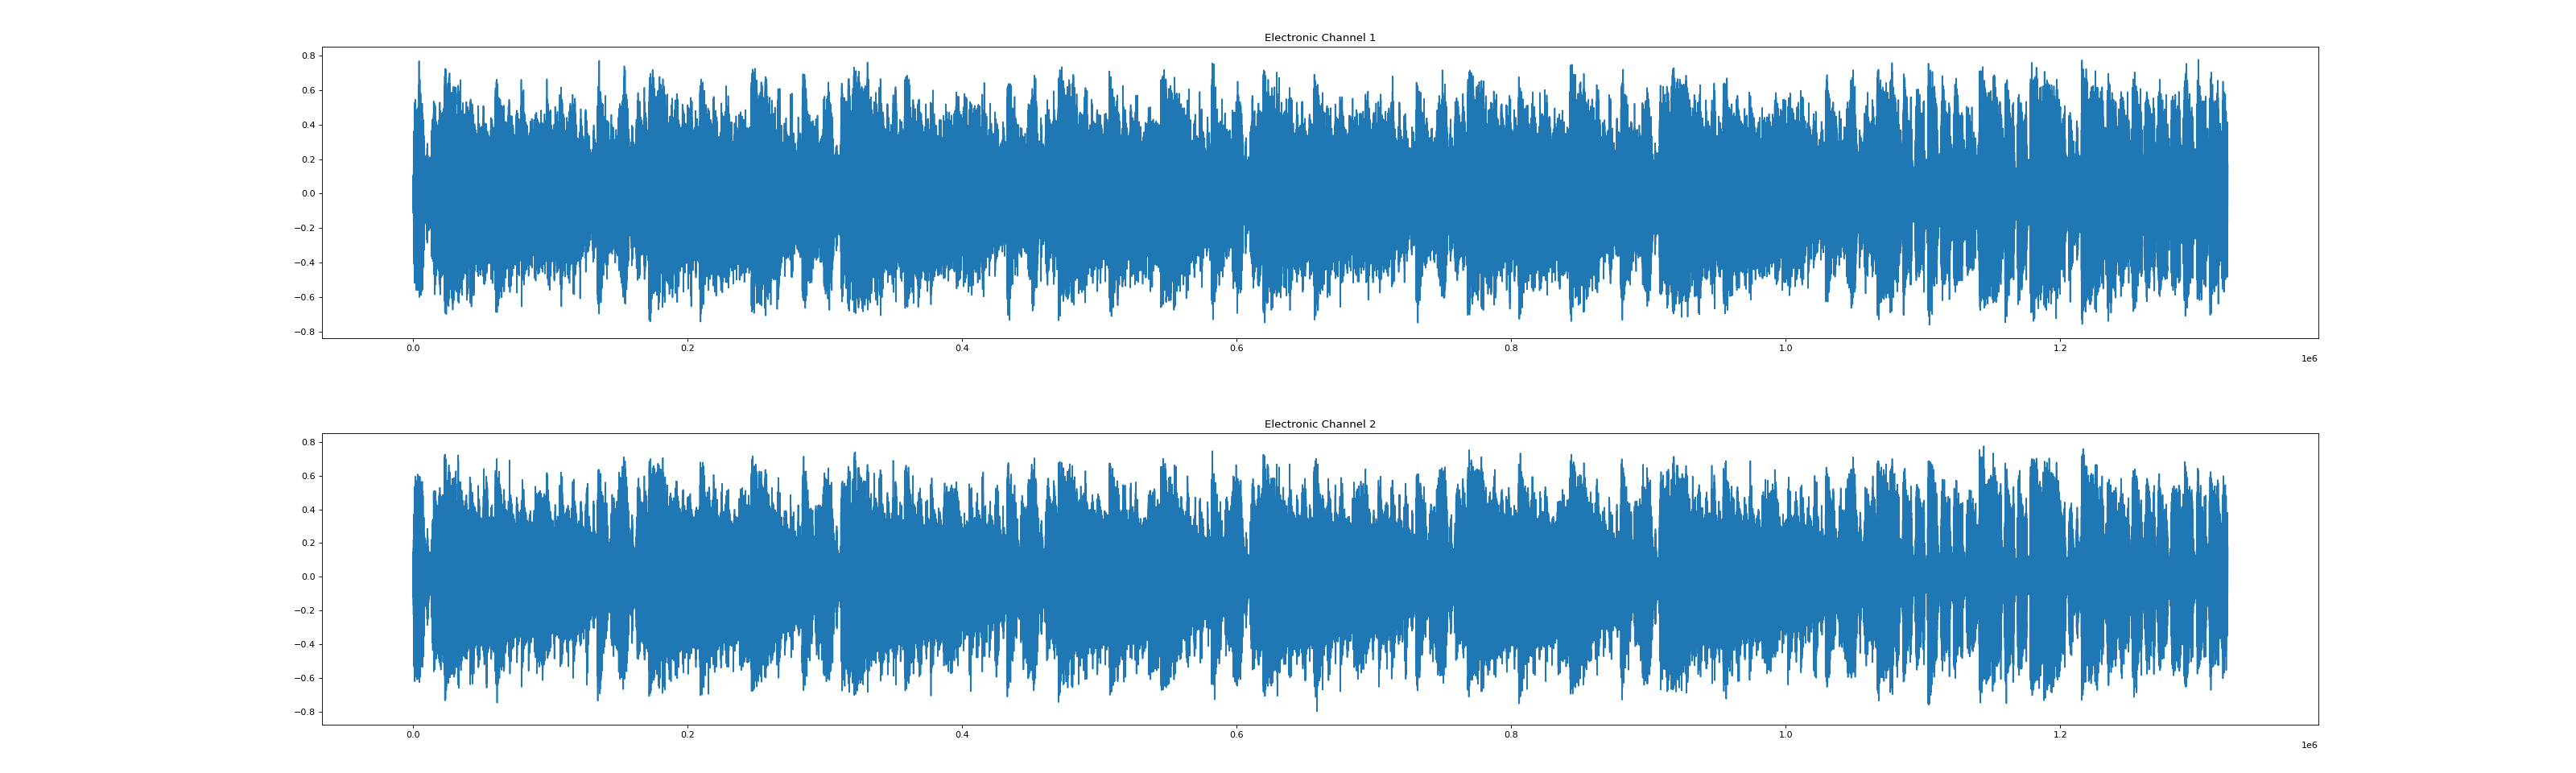
\includegraphics[width=\columnwidth]{../figures/overviews/Electronic.png}
  \caption{Electronic}
  \Description{Signals for Electronic Music}
  \label{fig:elec}
\end{figure}
\begin{figure}
  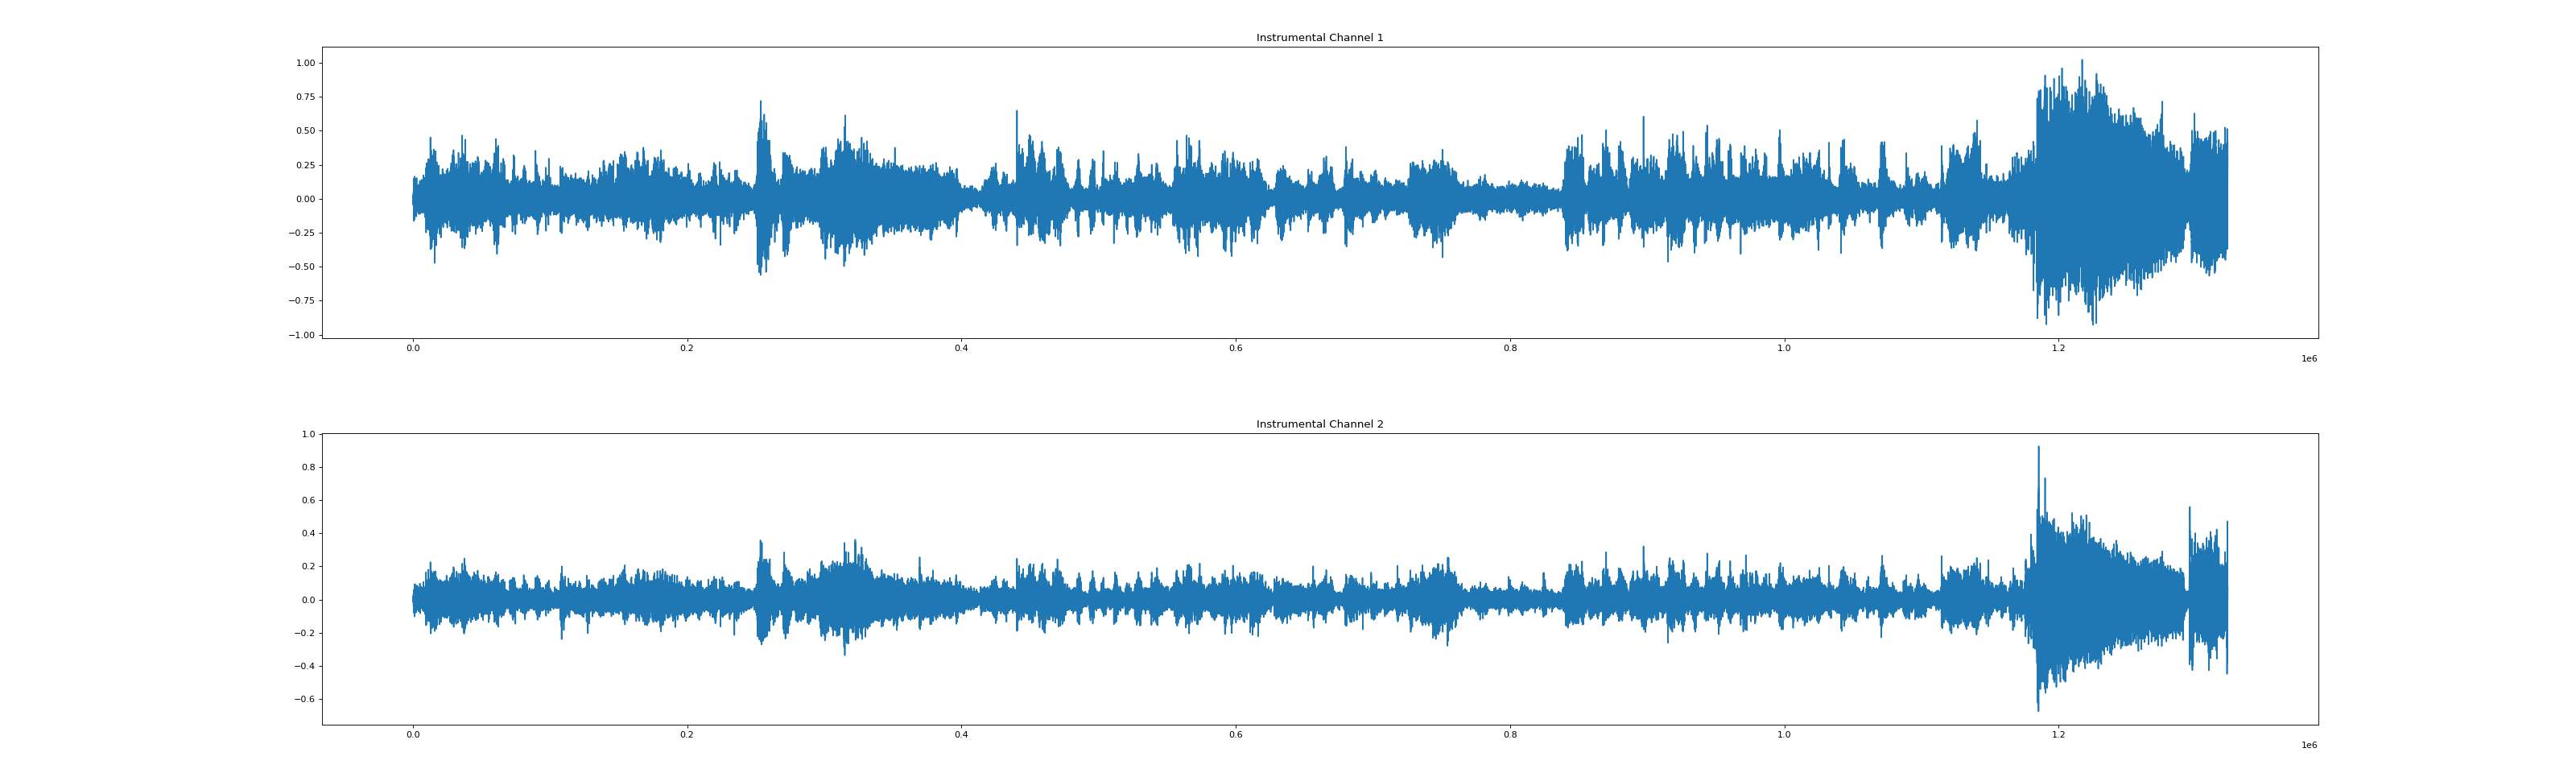
\includegraphics[width=\columnwidth]{../figures/overviews/Instrumental.png}
  \caption{Instrumental}
  \Description{Signals for Instrumental Music}
  \label{fig:intru}
\end{figure}

\section{Features}
Common audio features are used in this project, including beats, tuning, zero-crossing rate, autocorrelation, RMS, centroid, flatness, MFCC, and STFT.

\subsection{Feature Extraction}
The entire feature extraction process was completed with the LibROSA library \cite{brian_mcfee_2022_6097378}. The audios are loaded into signals with a sampling rate equal to 22050 and all the signals are resized into lengths equal to 660000 by either padding with 0 or clipping. The correlation between two channels is first calculated, and the following features are extracted only from the first channel. A series of audio signal $s$ can be decomposed into the sum of harmonic signals, $s_h$, with persuasive signals, $s_p$, namely $s = s_h+s_p$. 

Beats number and zero-crossing rate is then extracted from $s$, $s_h$ and $s_p$. Estmimated tuning is calculated for $s$. RMS, centroid, and flatness are calculated from all three signals. The mean and standard deviation values of these three features generated from all three signals are collected with additionally the max and min values generated from $s$ only. 20 MFCCs are calculated from $s$, and the max, min, mean and standard deviation values are collected. STFT is calculated with FFT window size equals 8 and the number of chroma equals 12. Only the first 20 columns of STFT are collected due to the consideration of computational costs. Finally, autocorrelations of $s$ are calculated with 4 different starting points. 

Table \ref{tabel:feature size} shows the number of features extracted from each audio.

\begin{table}[]
\begin{tabular}{r|c}
       & num of Features \\ \hline
Beats, Zero Crossing Rate  & $3\times2 = 6$ \\
Tuning & 1 \\
RMS, Centroid, Flatness & $2\times(3\times 3) +2\times 3 = 24 $ \\
MFCC & $20\times4 = 80$ \\
STFT & $12\times20 = 240$ \\
Autocorrelation & 4\\
\textbf{Overall} & \textbf{356}
\end{tabular}
\caption{Summary of extracted features}
\label{tabel:feature size}
\end{table}

\subsection{Feature Selection}
Considering the Random Forest will be used to classify the data points, the number of features would affect the performance. Thus, the following steps aimed to investigate the distinguishability of features and the correlations between each feature.

The value of a feature should vary between genres in order to allow the model to learn the difference otherwise it would be helpful. Two box plots are generated for each of the main features to investigate the effectivity with one including outliers and one that does not. The main features include the beat, tuning, zero-crossing rate, correlation, as well as the mean value of RMS, centroid, and flatness. As shown in Figure \ref{fig:beat}, beats do not show an obvious difference among most genres, while the remainings do, for example, the zero-crossing rate shown in Figure \ref{fig:zero crossing}. According to the consideration that beats are the fundamental feature of music, this feature has still remained. Based on the box plots, the extracted features are generally effective in the classification task. 

\begin{figure}[b]
  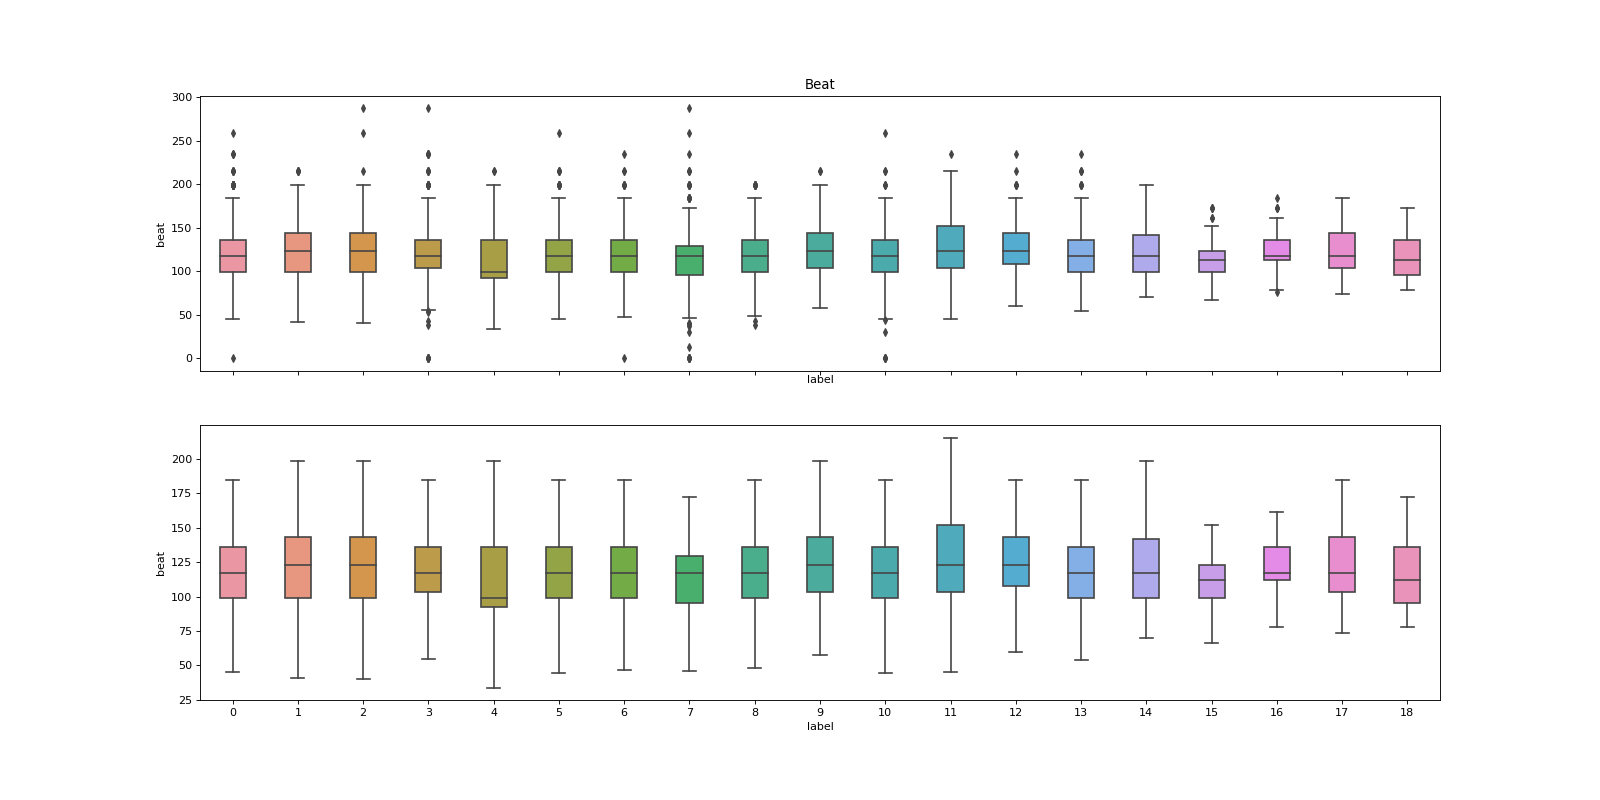
\includegraphics[width=\columnwidth]{../figures/Beat.png}
  \caption{Beats: Feature without obvious different}
  \Description{beats boxplot}
  \label{fig:beat}
\end{figure}
\begin{figure}[b]
  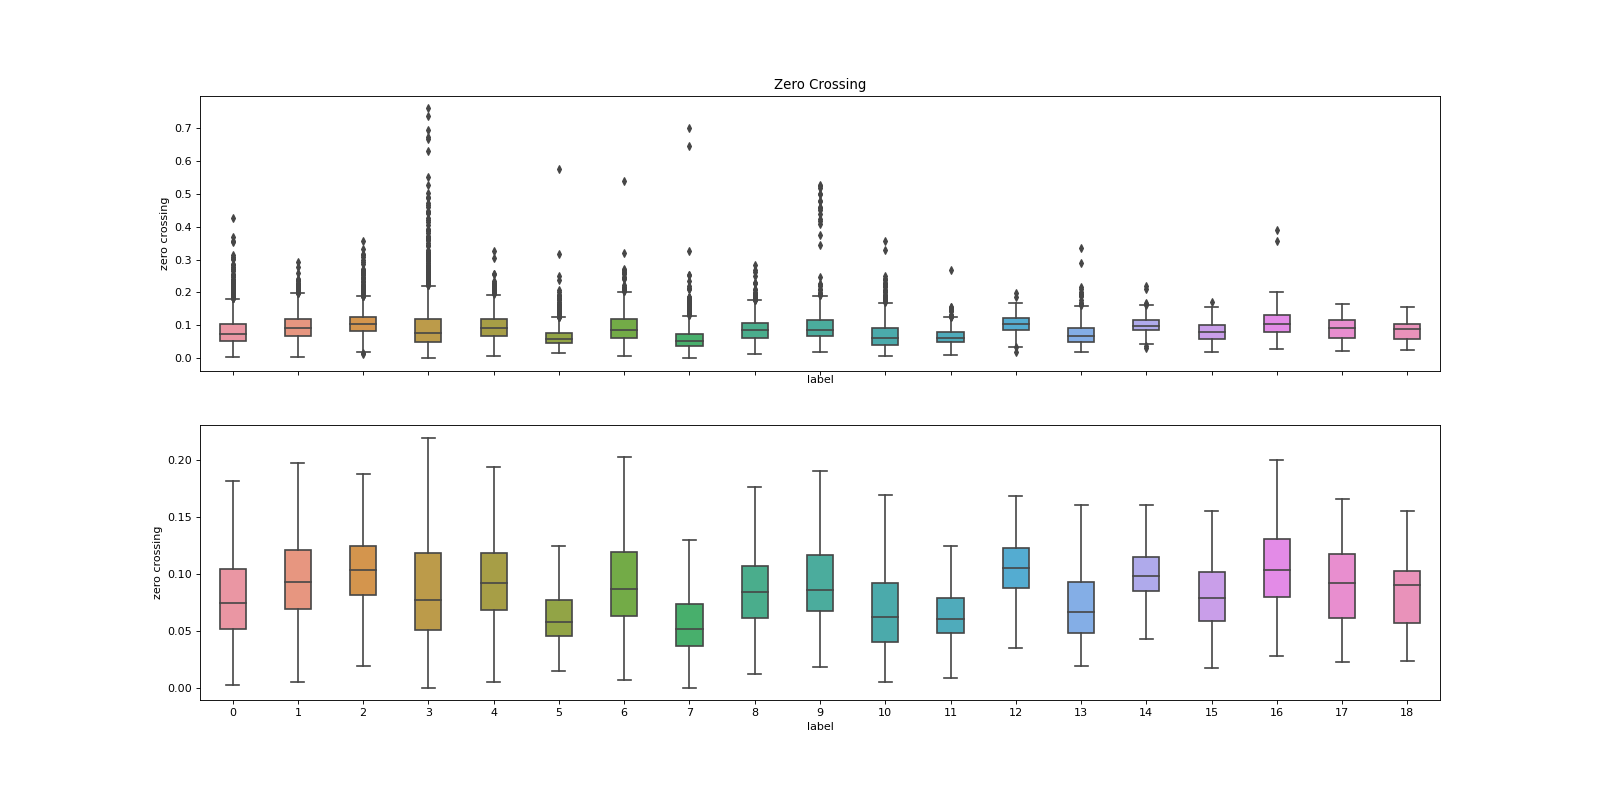
\includegraphics[width=\columnwidth]{../figures/Zero Crossing.png}
  \caption{Zero Crossing Rate:  Feature with obvious different}
  \Description{zero crossing rate boxplot}
  \label{fig:zero crossing}
\end{figure}

Besides the consideration of distinguishability of features, the correlation between features is another concern in selecting features. The goodness of a feature in the classification task can be summarized as the feature should be highly correlated with the labels while detached from other features \cite{yu2003feature}. Yu and Liu (2003) provided two effective methods to solve the problem of correlation, but due to the limits of computational power, in this project, the correlated features are filtered simply by randomly selecting one feature from the pair with a correlation higher than 0.8. Figure \ref{fig:corr} is the heatmap of the correlation between features. The bright red and bright blue area represents the questionable features with high correlations. In genreral, autocorrelations are highly correlated which forms the most questionable pairs. The columns of STFT and the standard deviation of MFCCs are also hightly correlated.

\begin{figure}
  \includegraphics[width=\columnwidth]{../figures/correlation.png}
  \caption{Heatmap representation of correlations}
  \Description{correlations}
  \label{fig:corr}
\end{figure}


\subsection{Generate Preprocessed Dataset}
Denote the dataset with 356 features generated from each audio as \textbf{Origin}. Beacuse the original value of features varies from $10^{-2}$ to $10^3$, a normalization of the features would improve the performance by shifting the attention away from the features with larger values. Assume ${\bf x}$ is a feature, then the normalization is achieved by:
\begin{align*}
{\bf z} = \frac{{\bf x}-{\bf x}_{min}}{{\bf x}_{max}-{\bf x}_{min}}
\end{align*}
After normalizing with this equation, values of all features are in the range of 0 to 1. Denote the normalized dataset as \textbf{Norm}. Finally,  the highly correlated features are filtered from the normalized dataset, and the remaining dataset is stored as \textbf{Filter}. The dimensions of these three datasets are listed in Table \ref{tabel:dataset}.

\begin{table}[b]
\begin{tabular}{r|c|c}
       & Dim & Range \\ \hline
origin & (19909, 356) & (0.01, 3200)\\
norm & (19909, 356) & [0,1]\\
filter & (19909, 193) & [0,1]
\end{tabular}
\caption{Dimension and Range of each dataset}
\label{tabel:dataset}
\end{table}

In order to further analysis whether the normalization and filteration affect the performance of classification, the three datasets are applied to a unsupervised clustering method, k-means. The results from k-means are compared with the ground truth label with the Jaccard score, where
\begin{align*}
Jaccard = \frac{|X \cap Y|}{|X \cup Y|}.
\end{align*}
The results are shown in Table \ref{tabel:kmean}. From the results, the normalized dataset outperforms the original one, and the filtered dataset outperforms the non-filtered one. Thus, I would expect that the \textbf{Filter} outperforms others in the supervised classification task.

\begin{table}[]
\begin{tabular}{r|c|c|c}
 genre\_id & \textbf{Norm} &\textbf{Origin}&\textbf{Filter}\\ \hline
 0 &\textbf{0.146819}&0.108962  &0.137913  \\
 1 &0.119828  &0.120253  &\textbf{0.137296}\\
 2 &0.141254  &0.120257  &\textbf{0.186090}\\
 3 &0.098007  &\textbf{0.128776}&0.080893  \\
 4 &\textbf{0.192417}&0.099583  &0.161937  \\
 5 &0.108278  &0.095206  &\textbf{0.153144}\\
 6 &0.065004  &0.057158  &\textbf{0.098481}\\
 7 &0.099402  &0.075729  &\textbf{0.108641}\\
 8 &\textbf{0.056432}&0.045413  &0.049636  \\
 9 &0.085329  &0.056055  &\textbf{0.086779}\\
10 &\textbf{0.057931}&0.040620  &0.054520  \\
11 &\textbf{0.143411}&0.055924  &0.118032  \\
12 &0.292079  &0.047026  &\textbf{0.473267}\\
13 &0.030270  &0.021597  &\textbf{0.0608}  \\
14 &0.016350  &0.009717  &\textbf{0.019933}\\
15 &0.011255  &0.009434  &\textbf{0.014237}\\
16 &0.016536  &0.010711  &\textbf{0.023174}\\
17 &0.005904  &0.004182  &\textbf{0.006872}\\
18 &0.003693  &0.002240  &\textbf{0.004418}S
\end{tabular}
\caption{Jaccard scores of k-means}
\label{tabel:kmean}
\end{table}


\section{Experiments}
The three datasets are splited into training and testing pair with propotion 80\%/20\% in the same way, namely all the training datasets are the features from the same group of raw data, as well as the testing datasets. Each training dataset has 15,927 data points and each testing dataset has 3,982 data points. Specificlly, the testing dataset has 644 in Electronic, 627 in Rock, 554 in Punk, 341 in Experimental, 311 in Hip-Hop, 250 in Folk, 226 in Chiptune and Glitch, 210 in Instrumental, 185 in Pop, 162 in International, 163 in Ambient Electronic, 86 in Classical, 80 in Old-Time and Historic, 57 in Jazz, 32 in Country, 17 in Soul-RnB, 18 in Spoken, 17 in Blues, and 2 in Easy Listening.

\begin{figure*}
  \includegraphics[width=\textwidth]{../figures/labeled res.png}
  \caption{"One over rest" evaluations for 19 genres on 2 models and 3 feature sets}
  \Description{ovr}
  \label{fig:ovr res}
\end{figure*}

\subsection{Models}
Two models are used in this project, Random Forest and CNN. In order to improve the performance of RF, 10 different RF are grown on the same training data to predict the testing data. The final result is formed from a majority vote. 
The CNN is structured with 2 Conv1D layers, a batch normalization layer, a dropout layer with a 0.5 dropout rate, a flatten, and then a dense layer to shape (,100), and finally the output layer with output shape (,19). 

\subsection{Evaluation Metrices}
The evaluation is based on accuracy, F1\_score, precision, recall and AUC score. Evaluations of both overall (Table \ref{tabel:gene eval}) and labels indivisually (Figure \ref{fig:ovr res}) are provided. 

\begin{table}[h]
\begin{tabular}{r|c|c|c|c|c}
  & ACC &F1&Precision & Recall& AUC \\ \hline
RF\_origin & 0.4588 & 0.3315 & \textbf{0.5050} & 0.3230 & \\
RF\_norm & 0.4555 & 0.3295 & 0.5019 & 0.3207 & \\
RF\_filter & 0.4671 & 0.3339 & 0.4929 & 0.3265 & \\
CNN\_Origin & 0.3787 & 0.2240 & 0.3174 & 0.2269 & 0.8311 \\
CNN\_Norm & 0.4591 & 0.3243 & 0.3920 & 0.3176  & 0.8616 \\
CNN\_filter & \textbf{0.4761} & \textbf{0.3543} & 0.4047 & \textbf{0.3528} & \textbf{0.8707}
\end{tabular}
\caption{General Evaluations}
\label{tabel:gene eval}
\end{table}

All the evaluation values are calculated as the average of the performance over 5 times execution. The confusion matrix of the best accuracy example of each model and feature set combination is also generated, for example, the result of CNN\_filter is shown in Figure \ref{fig:cnn filter cm}.

\begin{figure}[b]
  \includegraphics[width=\columnwidth]{../figures/keras_filter.png}
  \caption{Confution Matrix of CNN\_filter}
  \Description{correlations}
  \label{fig:cnn filter cm}
\end{figure}


\section{Discussion}

As shown in Figure \ref{fig:ovr res}, CNNs generally perform better than RFs. Within CNNs, the filtered feature set performs the best, then follows the normalized feature set, and the original one performs the worst. Among RFs, though using filtered features shows slight improvement, no apparent differences are presented in the results from original and normalized feature sets. This invariance may be due to the specific property of RF that it makes decisions based on tree-like formate instead of based on weights in linear models. Moreover, the last 5 lines, representing genres Country, Soul-RnB, Spoken, Blues, and Easy Listening, are mostly zeros representing the lack of capability in classifying these genres. This limitation may be because of the lack of training data in these genres, namely the number of all these genres is only about 2\% of the entire training dataset. This problem could be solved by either collecting more music from these genres or merging them into other more common genres.

The best accuracy achieved in this project is around 47.5\%. Although this accuracy is better than several models in classifying music into more than 10 genres \cite{comparison}, and its AUC score is similar to that of the CRNN model tasked to classify into 20 genres \cite{crnn}, it is much lower than the accuracy higher than 80\% achieved by previous research on GTZAN database \cite{lee2009automatic,fu2010feature,li2010automatic}. This relatively low performance would be explained by several reasons, including (i) the genres are human-annotated which contain errors, (ii) the dataset is highly imbalanced on several genres, (iii) the possible features are not fully contained, for example, STFT and MFCCs, because of the consideration of the computational capability of the device and (iv) the structure of the CNN is too simple to be robust.


Besides the problem on the dataset itself, others could be improved in future work. The STFT and MFCC features could be pre-trained with CNN to extract features to reduce the dimension \cite{fu2010survey,dieleman2011audio}, instead of achieving the goal by simply dropping the columns in this project. Other audio features could also be considered, for example, the rhythmic content features promoted by Tzanetakis et al. (2002) \cite{gtzan}. In \cite{valero2012gammatone}, Valero and Alias announced that the Gammatone Cepstral Coefficients (GTCC) is more powerful than MFCC when facing classification tasks, so GTCC may be investigated in the future research. Moreover, according to Dielman and Schrauwen (2014), the pooling layer is inappropriate in this music classification context \cite{endtoend}. Thus, the CNN structure could be improved by removing the pooling layer, adding more convolutional layers or dense layers, or changing the shape of outputs in the hidden layers. 


\section{Conclusion}

This project aimed to develop models on classify music into more than 10 genres. The dataset used in this project is found on Kaggle, which contains 19.9 labeled music segments in the 30s. Audio signal features are extracted from the raw data, and, by different pre-processing steps, transformed into three different feature sets. Two models, Random Forest and 2-Layer CNN were then built to classify the music based on these feature sets and achieved the best accuracy higher than 47\%. After investigating the evaluations, the limitations of this project are summarized. The limitations include (i) the questionable label quality and the imbalance that occurs in the raw dataset, (ii) the dropoff during the feature extraction, and (iii) the structure of the classifiers. Future research will aim to solve this problem and achieve a better-performed model on music genre classification.
    


\bibliographystyle{ACM-Reference-Format}
\bibliography{ref}{}
\end{document}